\documentclass[8pt,a4paper,french]{article}
\usepackage[margin=0.75in]{geometry}
\usepackage{babel}
\usepackage[T1]{fontenc}
\usepackage{graphicx}
\usepackage{tocloft}
\usepackage{array}
\usepackage{enumitem}
\usepackage{wrapfig}
%% https://www.overleaf.com/learn/latex/Using_colors_in_LaTeX
\usepackage[dvipsnames]{xcolor}
%% https://latex-tutorial.com/bullet-styles/
\usepackage{pifont}

\renewcommand{\familydefault}{\sfdefault}

\newcommand{\amap}{Association Maintien Agriculture Paysanne (AMAP)}

\newcommand{\defineauthorcolor}[2]{%
  \colorlet{author#1}{#2}% Create an author colour
  \expandafter\def\csname authoredby#1\endcsname{% Create author colour settings
    %% \renewcommand{\cftchapfont}{\bfseries\color{author#1}}% Chapter colour
    \renewcommand{\cftsecfont}{\color{author#1}}% Section colour
    \renewcommand{\cftsubsecfont}{\color{author#1}}% Subsection colour
    \renewcommand{\cftsubsubsecfont}{\color{author#1}}}% Subsubsection colour
}
\newcommand{\authoredby}[1]{\addtocontents{toc}{\protect\@nameuse{authoredby#1}}}%
\defineauthorcolor{A}{ForestGreen}% Author A will be coloured forest green
\defineauthorcolor{B}{Red}% Author B will be coloured red
\defineauthorcolor{C}{BlueGreen}% Author B will be coloured red

\usepackage{hyperref}
\hypersetup{
  colorlinks=true,
  linktoc=all,
  linkcolor=blue,
  linktocpage=true,
  pdfauthor = {\amap},
  pdfkeywords = {Agriculture, Paysanne},
  pdfcreator  = \LaTeX,
  pdfproducer = \LaTeX,
  pdftitle = {\amap},
  pdfsubject = {\amap},
  pdfpagemode = UseNone
}

\usepackage{titlesec}
\titleformat{\section}
{\color{ForestGreen}\normalfont\Large\bfseries}
{\color{ForestGreen}\thesection}{1em}{}
\titleformat{\subsection}
{\color{Red}\normalfont\Large\bfseries}
{\color{Red}\thesubsection}{0.75em}{}
\titleformat{\subsubsection}
{\color{BlueGreen}\normalfont\Large\bfseries}
{\color{BlueGreen}\thesubsubsection}{0.50em}{}

\begin{document}

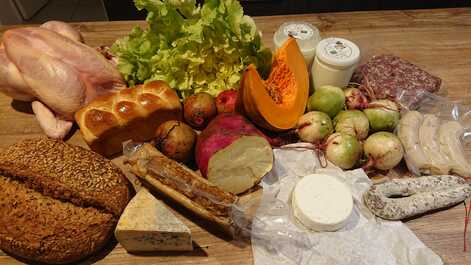
\includegraphics[width=0.3333\textwidth]{Gauche.jpg}
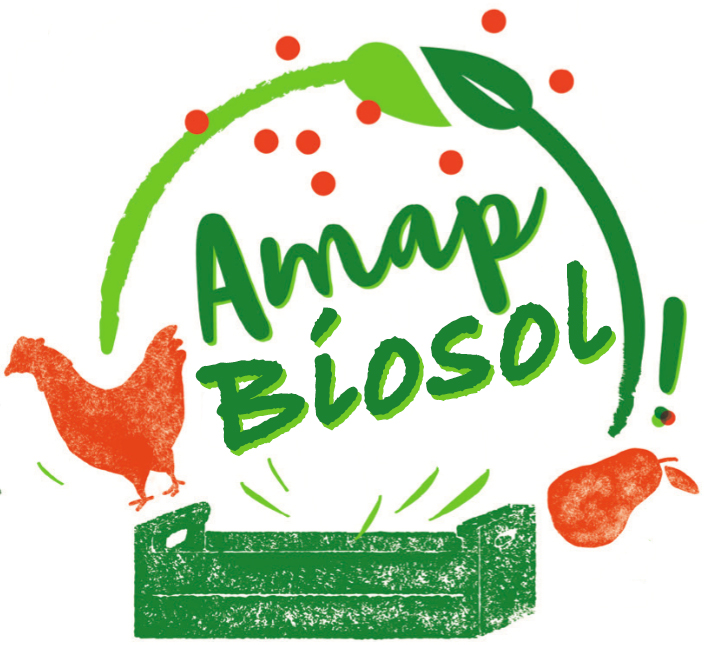
\includegraphics[width=0.3333\textwidth]{Centre.jpg}
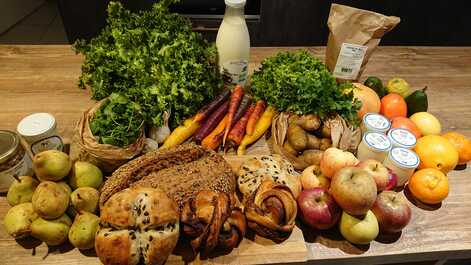
\includegraphics[width=0.3333\textwidth]{Droite.jpg}
\vspace{30ex}

\begin{center}
{\bf\color{ForestGreen} LIVRET D'ACCUEIL {\the\year{}}}
\vspace{1ex}

Dans un panier de savoir-faire et de savoir-être

Distribuer des aliments sans produits chimiques, sans OGM

Lier avec un partenariat équitable

Déglacer avec du lien social

Saupoudrer de convivialité

Si nécessaire, pimenter d'un coup de main sur la ferme

À partager sans modération !
\vspace{1ex}

{\small (Recette mijotée par l'AMAP de la Belle Terre)}
\vspace{30ex}


\includegraphics[width=0.3333\textwidth]{Ensemble.jpg}
\end{center}

\tableofcontents

\vspace{1em}
\noindent La source \LaTeX\ pour générer ce document se trouve à
\href{https://github.com/mdgabriel/amap/}{github.com/mdgabriel/amap/}.

%%%%%%%%%%%%%%%%%%%%%%%%%%%%%%%%%%%%%%%%%%%%%%%%%%%%%%%%%%%%%%%%%%%%%%%%%%%%%%%%

\authoredby{A}
\section{QU'EST-CE QU'UNE AMAP ?}\label{sec:amap}

\noindent Une \amap, c'est plus qu'un \guillemotleft\ panier \guillemotright !\newline

\noindent{\bf {\color{Red}A} comme {\color{Red}Association}}\newline
En AMAP, pas d'intermédiaire commercial. C'est le seul système qui
reverse 100\% du montant du panier à la paysanne ou au paysan. Ce sont
les amapiennes, les personnes engagées, qui s'organisent pour faire
vivre le partenariat.\newline

\noindent{\bf {\color{Red}M} comme {\color{Red}Maintien}}\newline
Chaque amapienne s'engage sur une saison : la paysanne ou le paysan a
l'assurance d'être rémunéré toute l'année pour son travail à un prix
juste et d'écouler sa production ! Cela permet de maintenir
l'agriculture paysanne dans nos régions.\newline

\noindent{\bf {\color{Red}AP} comme {\color{Red}Agriculture Paysanne}}\newline
L'AMAP soutient une agriculture de proximité, à taille humaine, qui
concilie protection de la nature, emploi agricole, pérennité des
fermes et qui rétablit le lien entre paysan-nes et mangeurs.\newline

\noindent Source : \underline{Réseau AMAP Île-de-France}\newline

\noindent Une AMAP est donc un partenariat de proximité entre une ferme et un
groupe de mangeurs qui s'engagent sur le long terme grâce à un
contrat.\newline

\noindent Vous êtes sur le point de rentrer dans une AMAP, vous allez donc
partager avec ce collectif de personnes des valeurs d'équité, de
solidarité et d'agriculture paysanne. Toutes ces valeurs et bien
d'autres encore ainsi que les principes découlant des AMAP ont été
formalisés dans la charte des AMAP, en annexe au livret, unissant
toutes les AMAP de France sur un socle commun.

%%%%%%%%%%%%%%%%%%%%%%%%%%%%%%%%%%%%%%%%%%%%%%%%%%%%%%%%%%%%%%%%%%%%%%%%%%%%%%%%

\authoredby{A}
\section{LA CHARTE}\label{sec:charte}

\noindent{\bf La charte inter-régionale des AMAP}\ : \href{https://amap-aura.org/la-charte-des-amap/}{https://amap-aura.org/la-charte-des-amap/}\newline

\noindent Les cinq principes fondamentaux\ :
\begin{enumerate}
\item Une démarche d'agriculture paysanne
\item Une pratique agro-écologique
\item Une alimentation de qualité et accessible
\item Une participation active dans une démarche d'éducation populaire
\item Une relation solidaire contractualisée sans intermédiaire
\end{enumerate}

%%%%%%%%%%%%%%%%%%%%%%%%%%%%%%%%%%%%%%%%%%%%%%%%%%%%%%%%%%%%%%%%%%%%%%%%%%%%%%%%

\authoredby{A}
\section{ET EN PRATIQUE ?}\label{sec:pratique}

\authoredby{B}
\subsection{Les contrats}\label{subsec:contrats}

\noindent L'AMAP est facilitatrice de contact : elle met en lien des
paysan-nes et des amapiennes. Le contrat encadre juridiquement le
partenariat. En général, un contrat est signé par paysan-ne.  Ces
contrats sont disponibles sur l'outil informatique
\href{https://www.clicamap.org/}{Clic'Amap}
(\href{https://www.clicamap.org/}{www.clicamap.org}).  Les contrats
sont gérés par les référents en relation avec chaque paysan-ne en
fonction des demandes.  L'amapienne décide de la périodicité du
règlement du contrat lors de sa validation.  Il existe des contrats
dits \guillemotleft\ flash \guillemotright correspondant à des
livraisons ponctuelles de produits telles que\ : huile d'olive,
agrumes, viandes\ ...

\authoredby{B}
\subsection{La distribution}\label{subsec:distribution}

\noindent La distribution est un temps fort dans l'AMAP. L'investissement de
chaque amapienne est nécessaire au bon déroulement de ce moment de
partage : aider les producteurs à décharger leurs produits, composer
les paniers, ranger et nettoyer la salle, etc.
L'outil \href{https://www.clicamap.org/}{Clic'Amap}
(\href{https://www.clicamap.org/}{www.clicamap.org})
prévient les amapiennes pour l'organisation de {\color{ForestGreen} la préparation des paniers qui se déroulent à 17H30}\ :
\begin{itemize}[label=\ding{226}]
\item {\bf Les amapiennes s'engagent à préparer les paniers 3 fois par an}
\item {\bf Elle a lieu chaque semaine le mercredi de 18h00 à 19H30 à la Maison des familles, 60 Impasse Gaston Teissier, VILLEFRANCHE SUR SAONE}
\item {\bf Pour toutes questions}\ : \href{mailto:amap-biosol@mailo.com}{amap-biosol@mailo.com}
\end{itemize}

\noindent La distribution s'organise de la manière suivante :
\begin{itemize}[label=\ding{226}]
\item Les amapiennes de permanence se chargent de préparer les paniers à l'avance
\item Chaque référent ou paysan-ne coche la prise des produits
\item Pour les légumes\ : le contenu des légumes est affiché 
\item A la fin de la distribution, une équipe de volontaires remet en place les tables et réalise un nettoyage rapide
\end{itemize}

\authoredby{B}
\subsection{Flexibilité}\label{subsec:flexibilité}

\noindent Pour les amapiennes
\begin{itemize}[label=\ding{226}]
\item Certains contrats prévoient la possibilité d'un échelonnement du règlement.
\item Certains contrats prévoient quelques absences aux distributions, retrouvez les conditions sur chaque contrat.
\item Possibilité de prendre un panier toutes les deux semaines, à la condition de créer un binôme pour alterner chaque semaine (vous inscrire à la liste d'attente pour trouver un partenaire de panier).
\item Des contacts entre amapiennes sont possibles en cas d'imprévus pour récupérer vos paniers (s'adresser au référent accueil).
\end{itemize}

\authoredby{B}
\subsection{Vie associative}\label{subsec:vieasso}

\noindent L'AMAP BIOSOL organise chaque année quelques rencontres, entre autres\ :
\begin{itemize}[label=\ding{226}]
\item Assemblée générale (début d'année) : elle permet de dresser le bilan de l'année écoulée et de déterminer les orientations à venir
\item Participation au forum des associations et à la fête de l'environnement
\item Visites chez les producteurs de l'AMAP
\item Coup de main aux paysan-nes
\item Portes ouvertes et pots conviviaux
\end{itemize}
    
%%%%%%%%%%%%%%%%%%%%%%%%%%%%%%%%%%%%%%%%%%%%%%%%%%%%%%%%%%%%%%%%%%%%%%%%%%%%%%%%

\authoredby{A}
\section{LES ACTEURS DE L'AMAP}\label{sec:acteurs}

\noindent La vie et la dynamique d'une AMAP, comme dans toutes associations,
dépendent de ses membres. Chaque amapienne a donc son rôle à jouer
dans une AMAP. Ci-après figurent les rôles et fonctions des acteurs de
l'AMAP ainsi que les personnes à contacter. N'hésitez pas à faire
appel à elles pour tout questionnement ou difficulté\ :

\authoredby{B}
\subsection{Les amapiennes}\label{subsec:amapiennes}

\noindent {\bf Venez rencontrer les amapiennes de notre association lors des distributions ou des rencontres organisées.}

\authoredby{B}
\subsection{La Collégiale}\label{subsec:collegiale}

\noindent {\bf Elle est constituée des référents \guillemotleft\ paysans \guillemotright et des référents \guillemotleft\ association \guillemotright.}

\authoredby{B}
\subsection{Les référents \guillemotleft\ association \guillemotright}\label{subsec:association}

\begin{center}
  \begin{tabular}{ p{3.75cm}|p{3.75cm}|p{3.75cm}|p{3.75cm} }
    {\bf Accueil} & {\bf Trésorier} & {\bf Communication} & {\bf Animation} \\
    \hline\hline
    Accompagne les nouvelles amapiennes & Gestion des adhésions & Mise à jour Clic'Amap, Facebook & Organisation des évènements \\
    \hline
    Martine CAUSSIN & Bernard MONTUELLE & Apolline LE RESTE, Amaury SCHMIT & Michèle MONTAGNIER \\
    
\includegraphics[width=1.5cm]{CAUSSIN.jpg} & 
\includegraphics[width=1.5cm]{MONTUELLE.jpg} & 
\includegraphics[width=1.5cm]{SCHMIT.jpg} & 
\includegraphics[height=2cm]{MONTAGNIER.jpg}
  \end{tabular}
\end{center}

\authoredby{B}
\subsection{Les référents \guillemotleft\ paysan-nes \guillemotright}\label{subsec:paysannes}

\noindent Les référents \guillemotleft\ paysans \guillemotright se chargent de tisser le lien entre amapiennes et paysan-nes. Ils élaborent les contrats avec les paysan-nes et collectent les règlements auprès des amapiennes
\vspace{1em}
\begin{center}
  \begin{tabular}{ p{3.75cm}|p{3.75cm}|p{3.75cm}|p{3.75cm} }
    {\bf Légumes} & {\bf Poulets et laitage brebis} & {\bf Laitage vaches/chèvre} & {\bf Pommes} \\
    \hline\hline
    Olivier JOOS, Florian FARGE & Lucas HOUEROU & Martine CAUSSIN & Hélène REDON \\
    
\includegraphics[height=1.9cm]{JOOS-FARGE.jpg} & 
\includegraphics[height=1.9cm]{HOUEROU.jpg} & 
\includegraphics[width=1.5cm]{CAUSSIN.jpg} & 
\includegraphics[height=1.9cm]{REDON.jpg}
  \end{tabular}
\end{center}
\vspace{1em}
\begin{center}
  \begin{tabular}{ p{3.75cm}|p{3.75cm}|p{3.75cm}|p{3.75cm} }
    {\bf Pain} & {\bf Charcuterie, veau, porc, oeufs} & {\bf Farines, pois chiches} & {\bf Tisanes et aromates} \\
    \hline\hline
    Danielle LEBAIL & Apolline LE RESTE & Jérôme SERME & Elodie PIVETEAU \\
    
\includegraphics[height=2.1cm]{LEBAIL.jpg} & 
\includegraphics[width=1.5cm]{LERESTE.jpg} & 
\includegraphics[height=2.1cm]{SERME.jpg} & 
\includegraphics[width=1.5cm]{PIVETEAU.jpg}
  \end{tabular}
\end{center}

%%%%%%%%%%%%%%%%%%%%%%%%%%%%%%%%%%%%%%%%%%%%%%%%%%%%%%%%%%%%%%%%%%%%%%%%%%%%%%%%

\authoredby{A}
\section{LES PAYSAN-NES DE L'AMAP}\label{sec:paysannes}

\noindent L'AMAP propose à ce jour des partenariats avec neuf
paysan-nes du secteur, dont voici les portraits.

\authoredby{B}
\subsection{Légumes --- LE JARDIN DES PIERRES DE SOLEIL}\label{subsec:legumes}

\begin{wrapfigure}[4]{L}{0.33\textwidth}
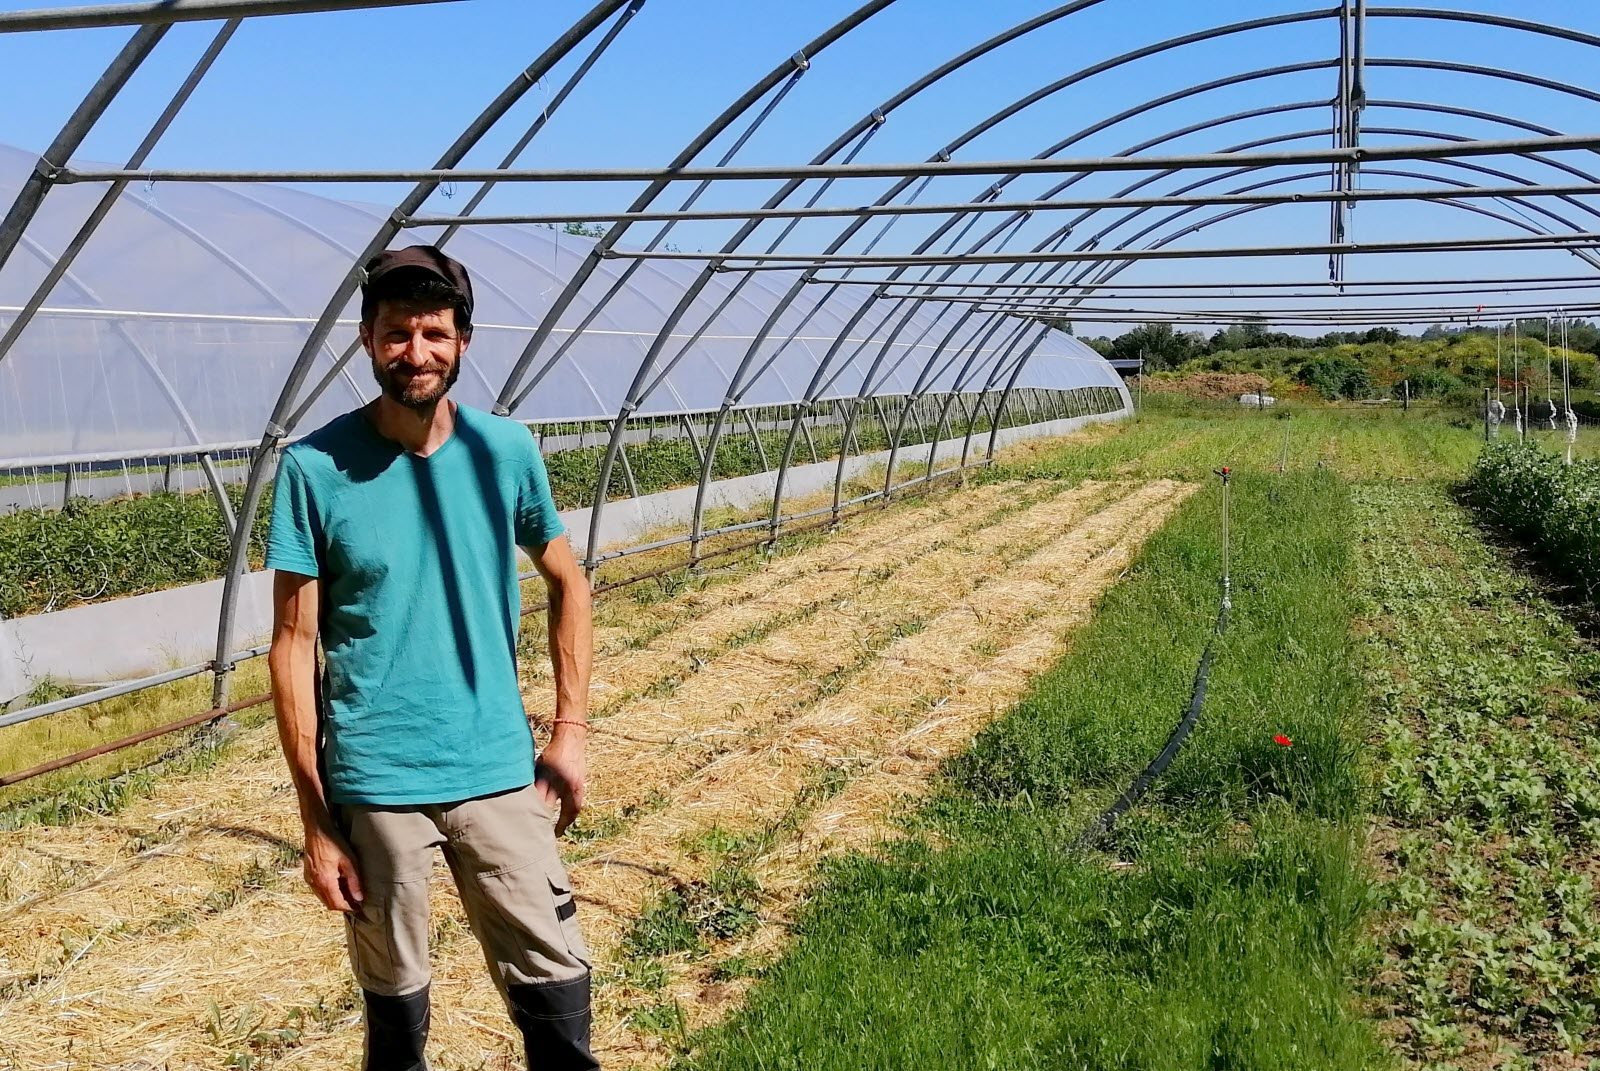
\includegraphics[width=0.3\textwidth]{LALAURE1.jpg}
\end{wrapfigure}

\noindent {\bf Pierre LALAURIE}\newline
494 du chemin de Port-Rivière\newline
01480 MESSIMY SUR SAONE\newline
Facebook\ : lesjardinsdespierresdesoleil\newline

\vspace{6em}

\begin{wrapfigure}[5]{R}{0.45\textwidth}
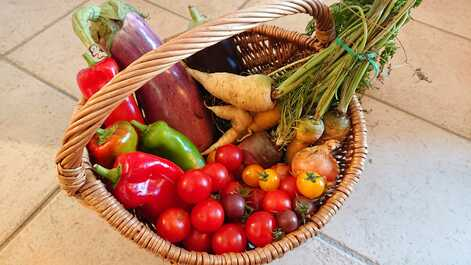
\includegraphics[width=0.4\textwidth]{LALAURE2.jpg}
\end{wrapfigure}
\noindent Micro-ferme maraîchère en bord de Saône cultivée en agriculture bio
d'un hectare se situe sur la commune de Messimy Sur Saône. Pierre est
installé depuis 2020 et propose trois tailles de paniers de légumes.
Pierre cultive une cinquantaine de variétés de légumes en suivant le
principe du maraîchage sur sol vivant (non travail du sol).

\vspace{10em}

\authoredby{B}
\subsection{Pommes --- CHEZ CHAMBE}\label{subsec:pommes}

\begin{wrapfigure}[20]{L}{0.4\textwidth}
\includegraphics[width=0.35\textwidth]{CHAMBE.jpg}
\end{wrapfigure}

\noindent {\bf Catherine HENRY, Olivier CHAMBE}\newline
325, route de Bel-Air\newline
69210 FLEURIEUX SUR L ARBRESLE\newline
\href{https://www.chezchambe.fr/}{www.chezchambe.fr}\newline

\noindent Sur les terres argileuses de Fleurieux et les sols sableux
de Lentilly, nous cultivons des légumes plein champ et sous serre, des
arbres fruitiers et des petits fruits, des céréales, des fleurs et des
sapins. Nos champs bénéficient de conditions idylliques\ : exposition
sud-est, vue sur les monts d'Or lyonnais, les Alpes à l'horizon, une
biodiversité préservée par les étangs, les bosquets, les prés ...\newline

\noindent Une entreprise familiale depuis 3 générations sur
actuellement 44 hectares. Depuis 2008, l'intégralité de la production
est certifiée agriculture biologique. \guillemotleft\ 80\% de ce qui
pousse sur terre prend vie dans les 30 premiers centimètres du
sol. Notre devoir est de préserver cet espace en nous interdisant tous
produits qui détruiraient en un seul passage l'activité microbienne
naturelle que nous protégeons au quotidien. \guillemotright\ Henry
CHAMBE

\newpage

\authoredby{B}
\subsection{Poulets, Laitage brebis --- A LA PETITE FERME DU PLAT}\label{subsec:poulets}

\begin{wrapfigure}[7]{L}{0.3\textwidth}
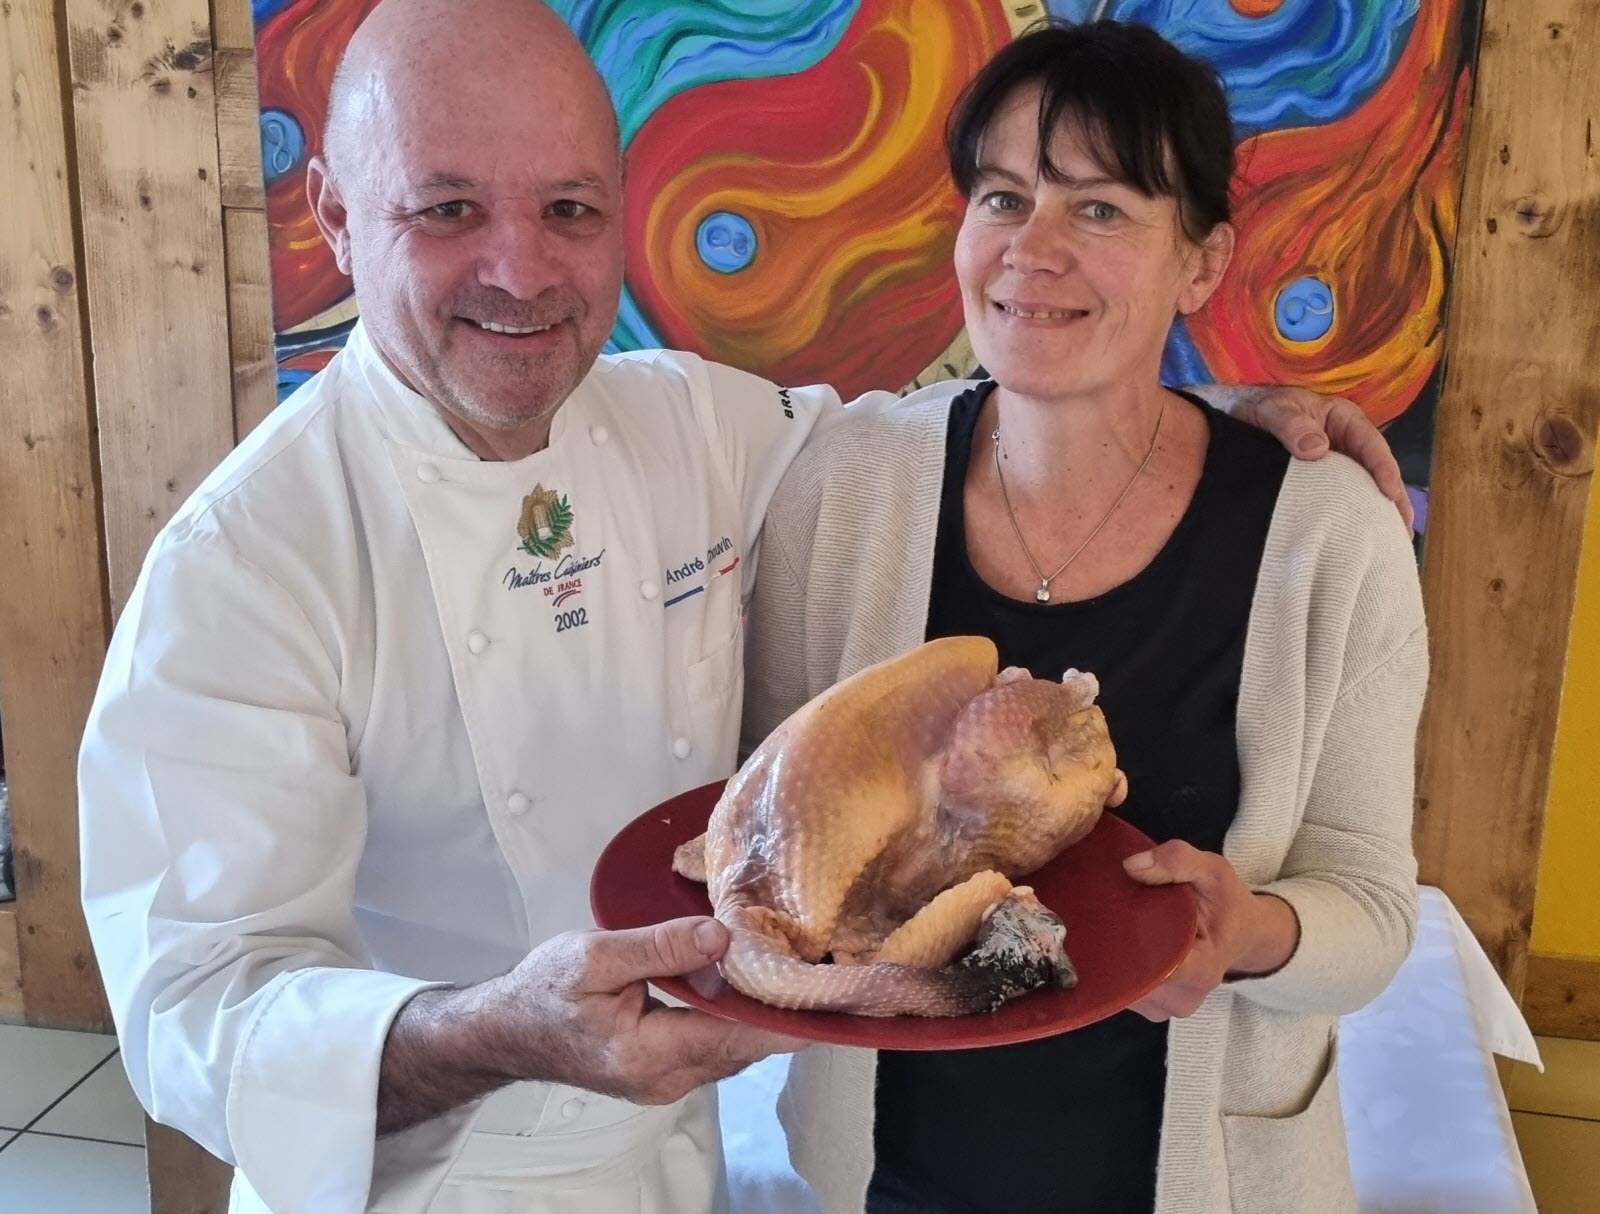
\includegraphics[width=0.25\textwidth]{GRILLET1.jpg}
\end{wrapfigure}

\noindent {\bf GRILLET Mireille}\newline
LE PLAT 69170 Saint-Clément-sur-Valsonne\newline

\noindent Installée en mai 2011 sur la ferme familiale sur les
hauteurs de Valsonne. Mireille a repris la ferme de ses parents en
2021 la faisant perdurer sur une troisième génération.\newline

\vspace{3em}

\begin{wrapfigure}[7]{R}{0.25\textwidth}
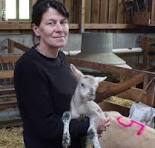
\includegraphics[height=0.2\textwidth]{GRILLET2.jpg}
\end{wrapfigure}

\noindent Aujourd'hui, Mireille Grillet est à la tête d'un cheptel
d'une soixantaine de brebis élevées en plein air, qui lui fournissent
viande et fromage. Par ailleurs, elle assure un élevage de poules
pondeuses, poulets, pintades, et volailles festives.\newline

\noindent Production de volailles fermières élevées sans OGM et ni antibiotique.\newline

\vspace{3em}

\authoredby{B}
\subsection{Poissons --- PISCICULTURE CHARLES MURGAT}\label{subsec:poissons}

\begin{wrapfigure}[5]{L}{0.25\textwidth}
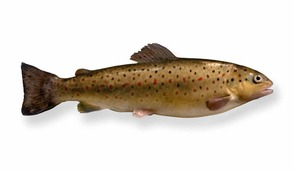
\includegraphics[width=0.2\textwidth]{Poissons1.jpg}
\end{wrapfigure}

\noindent 36 chemin du Lavoir - Les Fontaines 38270 Beaufort\newline
\href{https://www.charlesmurgat.com/}{www.charlesmurgat.com}\newline

\noindent Notre pisciculture est implantée, depuis 1898, au pied des
contreforts alpins, sur les sources naturelles des Fontaines de
l'Oron.

\vspace{2em}

\begin{wrapfigure}[5]{r}{0.25\textwidth}
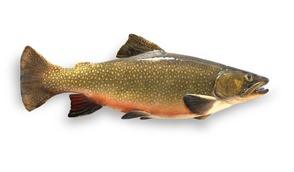
\includegraphics[width=0.2\textwidth]{Poissons2.jpg}
\end{wrapfigure}

\noindent Nous vous proposons une gamme de poissons frais, entiers ou
en filets. Nos Truites Fario, Ombles Chevaliers, Saumons de Fontaine
et Truites Arc-en-Ciel sont vidés et prêts à cuisiner.

\authoredby{B}
\subsection{{\OE}ufs, charcuterie, porc, veau --- LA GRANGE PRADEL}\label{subsec:oeufs}

\begin{wrapfigure}[4]{R}{0.45\textwidth}
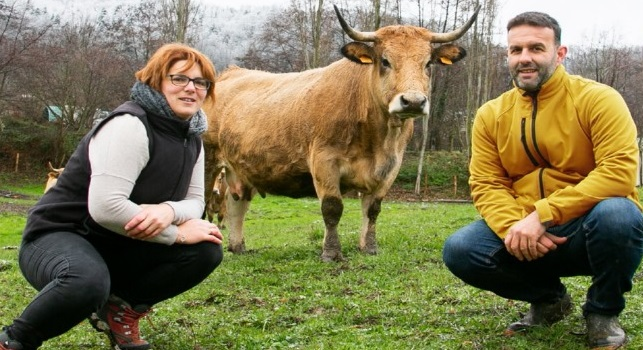
\includegraphics[width=0.4\textwidth]{MEUNIER1.jpg}
\end{wrapfigure}

\noindent {\bf Angélique et Laurent MEUNIER}\newline
La grange Pradel, 4033 route d'avauges\newline
69490 St Romain de Popey \newline

\vspace{9em}

\begin{wrapfigure}[8]{L}{0.45\textwidth}
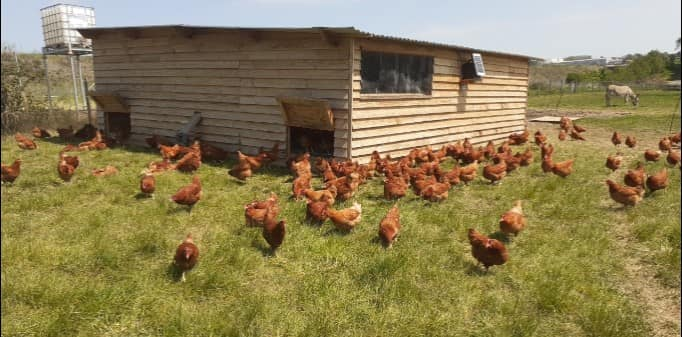
\includegraphics[width=0.4\textwidth]{MEUNIER2.jpg}
\end{wrapfigure}

\noindent Angélique et Laurent Meunier sont producteurs depuis 17 ans
et font partis de l'AMAP Biosol depuis le début. Ils sont producteurs
de poules pondeuses de plein air, éleveurs de porcs fermiers et de
vaches à viande. Ils ont sur l'exploitation un labo de transformation
où ils réalisent des charcuteries et des plats préparés. Ils proposent
des contrats d'{\oe}ufs, de charcuteries, de viande de porc et
régulièrement des ventes flashs de boeuf, veau et charcuteries de
saison.

\authoredby{B}
\subsection{Laitage vache et chèvre --- FERME TRIOMPHE}\label{subsec:laitage}

\begin{wrapfigure}[11]{L}{0.35\textwidth}
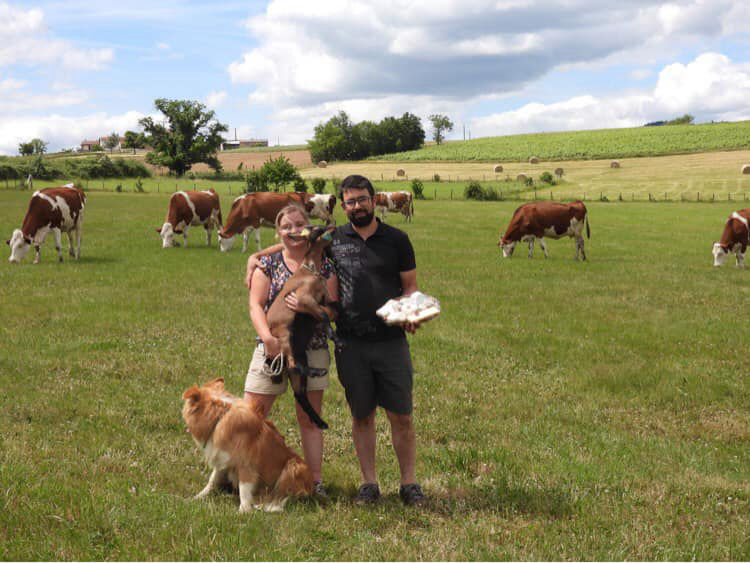
\includegraphics[width=0.3\textwidth]{TRIOMPHE1.jpg}
\end{wrapfigure}

\noindent {\bf Maêlys et Christophe}\newline
264 Impasse Triomphe\newline
69620 Saint-Vérand\newline
\href{https://fermetriomphe.fr/}{fermetriomphe.fr}\newline

\noindent En plein c{\oe}ur du Beaujolais, dans le village de Saint Vérand, à 30
minutes au nord de Lyon, entre vignes et forêts, se trouve la ferme
Triomphe.  Notre cheptel est constitué d'une trentaine de vaches
laitières et d'une vingtaine de génisses (jeunes femelles). Nos vaches
sont de race Montbéliarde, une race rustique qui produit un lait riche
et de qualité. Nos vaches pâturent de mars à novembre la bonne herbe
de nos prés autour de la ferme. Toute leur alimentation est produite
sur la ferme grâce à nos 45 hectares.  L'élevage\newline

\begin{wrapfigure}[11]{R}{0.35\textwidth}
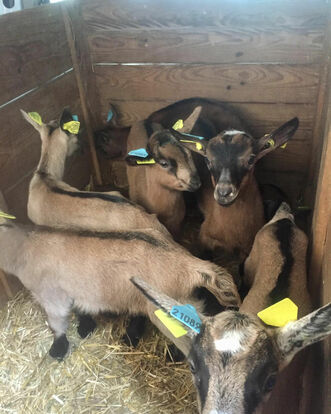
\includegraphics[height=0.3\textwidth]{TRIOMPHE2.jpg}
\end{wrapfigure}

\noindent de chèvres est la grande nouveauté pour 2022 ! Nous avons acheté une
cinquantaine de chevrettes de race Alpine Chamoisée qui ont été
élevées au lait de vache de la ferme.  Les chèvres sortent de mars à
novembre dans nos prés.  Nous respectons le cycle naturel des chèvres
et donc la quantité de lait produite baisse en début d'automne (début
de la reproduction) et s'arrête complètement de décembre à février
(fin de gestation) pour reprendre début février (c'est la saison des
mises-bas et des cabris).

\vspace{10em}

\authoredby{B}
\subsection{Farine --- LA FERME DES SOURCES}\label{subsec:farine}

\begin{wrapfigure}[14]{L}{0.45\textwidth}
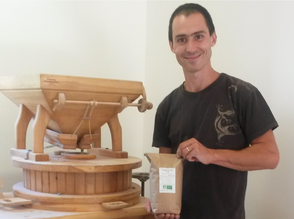
\includegraphics[width=0.4\textwidth]{BERNARD.jpg}
\end{wrapfigure}

\noindent {\bf Tonny BERNARD}\newline
{\bf Farine\ : blé, maïs, sarrasin et pois chiche}\newline
642, montée du moulin\newline 
01480 FAREINS\newline

\noindent\guillemotleft\ Après avoir fait des études de tourisme à
Lyon, je suis parti à Montpellier, puis dans l’Aveyron et à
Limoges. Je suis revenu dans mon village natal, à Fareins en 2012. J’y
ai planté mes racines en rénovant ma maison et en me formant à
l’agriculture auprès de mon père\ : un vrai retour aux sources !Je me
suis donc installé en 2017. Mon père a converti les terres en
agriculture biologique juste avant sa retraite en 2014. J’ai tout de
suite voulu un moulin pour valoriser les céréales que je cultive. Mon
idée étant de produire essentiellement une alimentation humaine, bio
et distribuée localement.  Je ne pratique pas le labour (ou TRES
exceptionnellement), et travaille le sol superficiellement. Je mise
beaucoup sur l’autonomie semencière, en y semant plusieurs variétés
anciennes de blé, de maïs, de petit épeautre – des variétés non
hybrides dites ‘population’. Je cherche autant que possible
l’autonomie paysanne ; je nettoie, trie, calibre, brosse et stocke mon
grain à la ferme, avec mes machines dont certaines sont
auto-construites. Le grain est moulu sur .meule de pierre, également à
la ferme.  Je préserve les haies qui bordent mes champs et mise au fil
du temps d’en replanter davantage…  Je fais de la farine à Fareins,
j’habite montée du moulin, le hangar est chemin des sources…  Tout ça
coule de source !!! \guillemotright

\newpage

\authoredby{B}
\subsection{Pain --- LE PAIN et JO}\label{subsec:pain}

\begin{wrapfigure}[13]{L}{0.45\textwidth}
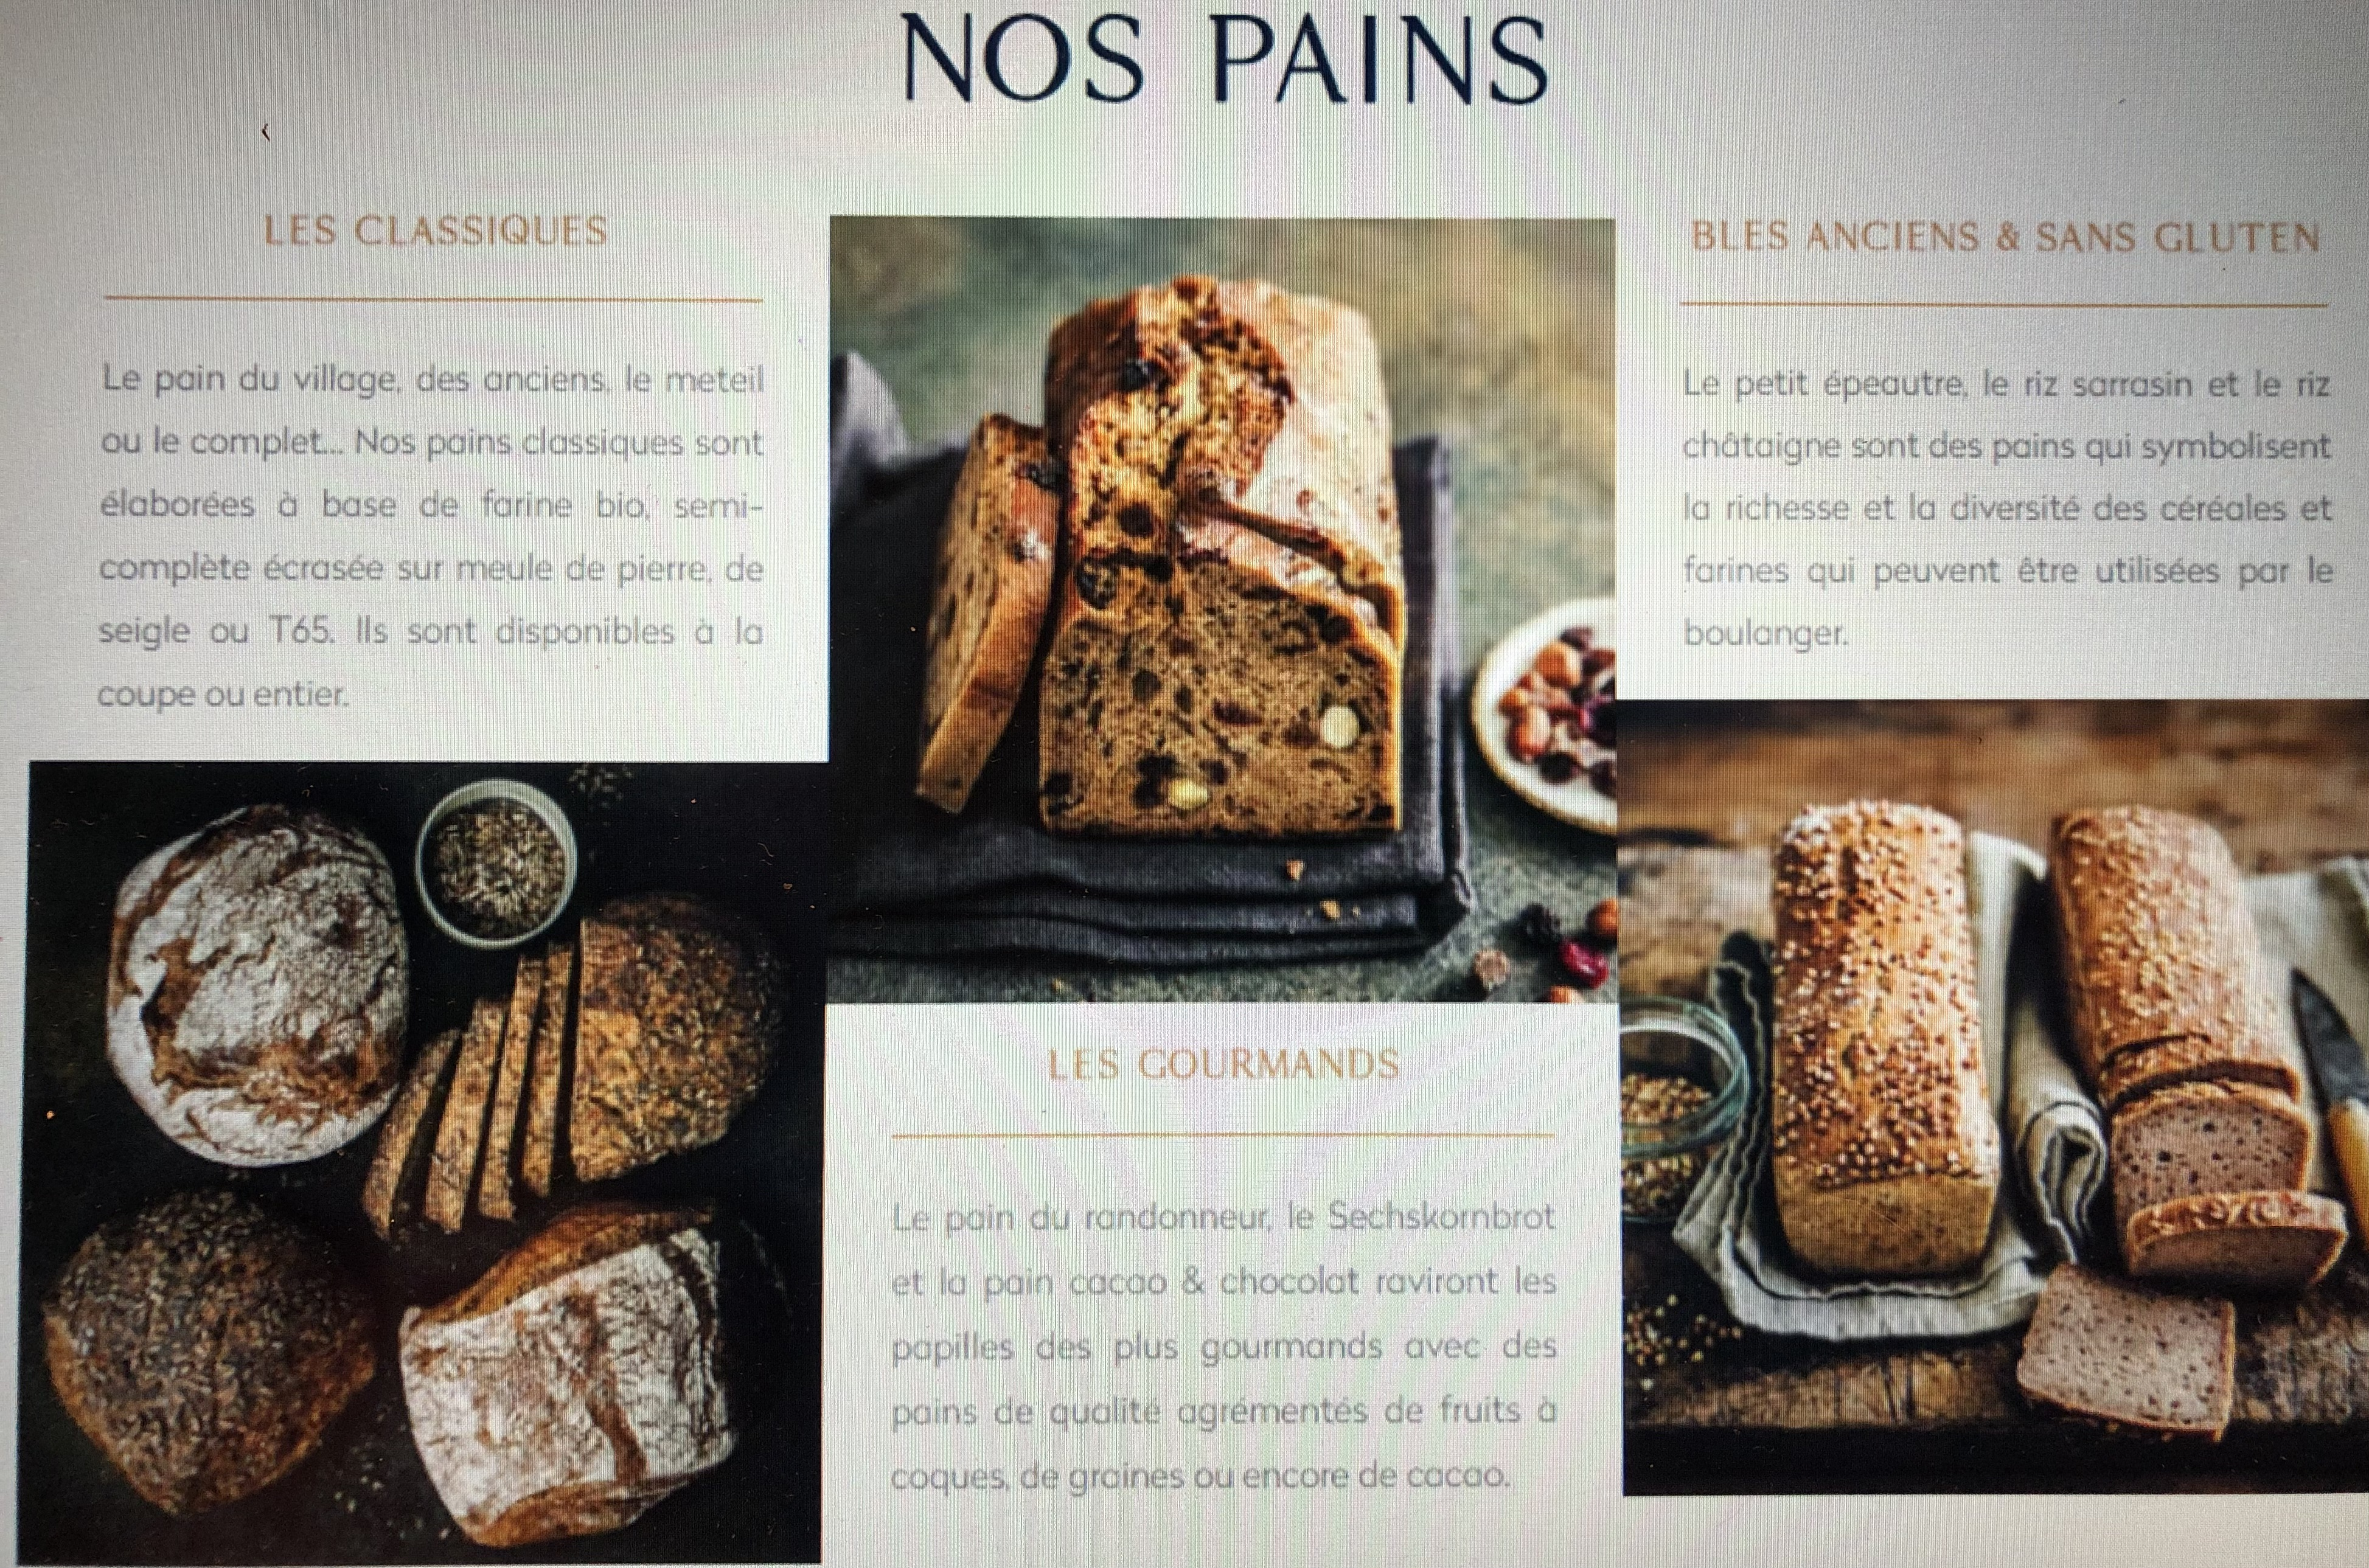
\includegraphics[width=0.4\textwidth]{Pain.jpg}
\end{wrapfigure}

\noindent 333 rue d’anse, 69 400 Villefranche S/S\newline
3 place de l’église, 69 480 Morancé \newline
\href{https://www.lepainetjo.fr}{www.lepainetjo.fr}\newline

\noindent À partir d’ingrédients bio, nos produits sont élaborés dans
le respect de la tradition et sont tous faits maison. Notre démarche
allie le respect de l’écologie et l’utilisation de produits locaux
pour la confection de nos produits salés et sucrés. Nous avons
sélectionné des farines Françaises issues de l’agriculture
biologique. Principalement écrasées à la meule de pierre, elles
permettent de préserver toutes les qualités nutritionnelles des
céréales.  Tous nos pains sont bio et réalisés à base de levain
naturel, pétris lentement et façonnés exclusivement à la main, dans le
pur respect des méthodes artisanales et traditionnelles. Le levain
naturel a beaucoup de vertus\ : il permet aux pains de se conserver sur
plusieurs jours, il apporte des bienfaits nutritionnels comme les
minéraux, donne plus de goût au pain et aussi, permet une meilleure
digestion du gluten naturellement présent dans le blé. Nous
travaillons exclusivement sur une fermentation lente et naturelle,
gage d’un pain très digeste et de bonne conservation. Ainsi, il nous
faut 2 à 3 jours pour faire nos pains. Ce qui est important des
préciser, c’est que nous n’avons rien réinventé. Nous travaillons
simplement comme le faisaient les anciens.

\authoredby{B}
\subsection{Tisanes et aromates --- JARDINS DE LA FORTUNE}\label{subsec:tisanes}

\begin{wrapfigure}[11]{L}{0.15\textwidth}
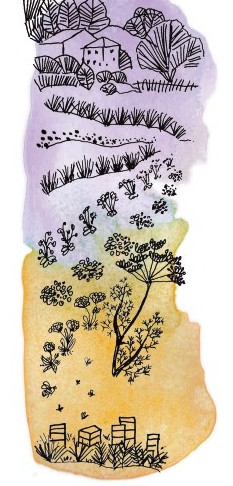
\includegraphics[height=0.25\textwidth]{Tisanes1.jpg}
\end{wrapfigure}

\noindent {\bf Béatrice Baron}\newline
779 Route de la fortune 69680 Poule les  Echarmeaux\newline
Facebook\ : jardinsdelafortune\newline

\noindent C'est en 2016, à Poule-les-Écharmeaux, au hameau de la
Fortue, que je me suis installée paysanne de plantes à tisanes et
condimentaires.  Les Jardins accueillent environ 40 plantes cultivées
dans le respect de l'environnent et de la biodiversité selon les
principales de l'{\bf agriculture biologique}.  Quelques plantes sont
simplement cueillies dans la nature localement.
Désherbage manuel, non-labour après la 1ère implantation, entretien de
la fertilité par l'apport de fumier composé\ : nos techniques de leur
qualité, les plantes sont récoltées et triées {\bf à la main}, et
j'apporte un grand soin à leur séchage et à leur conservation.
J'élabore une gamme de plantes sèches, {\bf tisanes}\newline

\begin{wrapfigure}[5]{R}{0.45\textwidth}
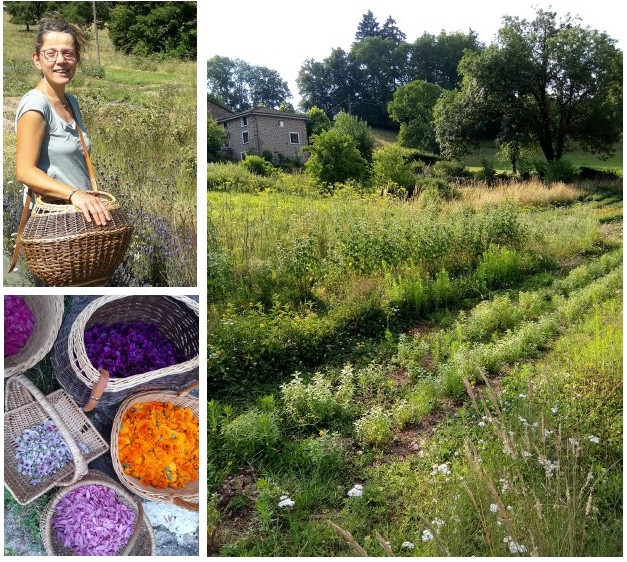
\includegraphics[width=0.4\textwidth]{Tisanes2.jpg}
\end{wrapfigure}

\noindent (en simple et en mélange) et {\bf aromates}, ainsi que des {\bf
  vinaigres et sels aux plantes}.  Soucieuse de vous proposer des {\bf
  produits d'exception}, je travaille à rendre les mélanges à la fois
beaux à l'oeil et goûteux au palais.  Saveur et couleur sont au
rendez-vous\ !

%%%%%%%%%%%%%%%%%%%%%%%%%%%%%%%%%%%%%%%%%%%%%%%%%%%%%%%%%%%%%%%%%%%%%%%%%%%%%%%%

\newpage

\authoredby{A}
\section{ANNEXE TARIFS CONTRATS 2023/2024}\label{sec:annexes}

\authoredby{B}
\subsection{Légumes --- Les jardins des Pierres de soleil}

\noindent Le contrat court du 8/11/2023 au 30/10/2024 et comprend 46 livraisons.\newline\newline
{\color{Blue} Grand Panier 19,00 €}\newline
{\color{Blue} Petit Panier 14,00 €}\newline
{\color{Blue} Mini panier 9,00 €}

\authoredby{B}
\subsection{Poulets, Laitage brebis --- À la petite ferme du plat}

\noindent Le contrat court du 22/02/2023 au 08/11/2023 et comprend 10 livraisons.\newline\newline
{\color{Blue} POULET / 1 Unité (2,2 kg) 23,30 €}\newline
{\color{Blue} POULET DECOUPE / 1 Unité (2,2 kg) 27,70 €}\newline

\noindent Le contrat court du 22/11/2023 au 17/07/2024 et comprend 13 livraisons.\newline\newline
{\color{Blue} sonnaille affiné / 3 unités 6,00 € }\newline
{\color{Blue} sonnaille - Aromatisé 3 parfums / 1 unité 4,80 € }\newline
{\color{Blue} Surprise Brebis / - 3,50 € }\newline
{\color{Blue} Sonnaille frais / 3 unités 6,00 € }\newline
{\color{Blue} sonnaille frais / 1 unité 2,20 € }\newline
{\color{Blue} sonnaille panachés (frais, affiné au choix)) / 3 (au choix) 6,00 €}\newline
{\color{Blue} sonnaille affiné / 1 unité 2,20 €}\newline
{\color{Blue} Yaourt Nature Brebis / 1 pot en verre de 400gr 3,60 €}\newline
{\color{Blue} Yaourt Nature Brebis (2 unités) / 2 pots en verre de 400gr 6,60 €}\newline
{\color{Blue} Yaourt Nature Brebis (3 unités) / 3 pots en verre de 400gr 9,00 €}

\authoredby{B}
\subsection{Poissons --- Pisciculture Charles Murgat}

\noindent Un contrat flash environ tous les trimestres.\newline\newline
{\color{Blue} Découverte (Filets de Truite Arc En Ciel, Truites Fario, Filet d'Omble Chevalier, Saumon de Fontaine) / Colis de 3.5 kg 58,00 € }\newline
{\color{Blue} Filet des Truites Arc En Ciel Saumonée / Colis 2 kg (env 8 filets) 37,00 € }\newline
{\color{Blue} Filets d'Omble Chevalier / Colis de 2 kg (env. 8 filets) 60€ }\newline
{\color{Blue} Filets de Truite Arc en Ciel Saumonée / Colis de 3 kg (env. 12 filets) 48,00 € }\newline
{\color{Blue} Filets de Truite Arc En Ciel Saumonée / Colis de 4 kg 58€ }\newline
{\color{Blue} Filets de Truites Fario / Colis de 2 kg (env. 8 filets) 48,00 € }\newline
{\color{Blue} Mix Filets (1kg Filet Truite saumonée, 1kg Filet Fario, 1kg Filet Omble Chevalier) / Colis de 3 kg 69,00 € }\newline
{\color{Blue} Oeufs de saumon de fontaine / pot de 90 g 8,00 € }\newline
{\color{Blue} Oeufs de Truite / Pot de 90 gr 8,00 € }\newline
{\color{Blue} Saumon de Fontaine / Colis de 3 kg (env. 10 poissons) 38€ }\newline
{\color{Blue} Truite arc en ciel à chair blanche / colis de 3kg 32,00 € }\newline
{\color{Blue} Truite arc en ciel à chair saumonée / colis de 3kg 33,00 € }\newline
{\color{Blue} Truite Fumée / 200 gr 13,00 € }\newline
{\color{Blue} Truites Blanches / Colis de 3 kg (env. 10 poissons) 32,00 € }\newline
{\color{Blue} Truites Fario / Colis de 3 kg (env. 10 poissons) 38,00 € }\newline
{\color{Blue} Chat --- Les Terrines de Lucien / 5 portions de 80 g 5,00 €}

\newpage

\authoredby{B}
\subsection{{\OE}ufs, charcuterie, porc, veau --- FERME  la Grange Pradel}

\noindent Charcuterie\ : Le contrat court du 24/04/2024 au 04/12/2024 et comprend 9 livraisons.\newline\newline
{\color{Blue} Panier Duo  avec gourmandise / 4 articles en moyenne 24,00 € }\newline
{\color{Blue} Panier Duo sans gourmandise / 3 articles en moyenne 21,00 € }\newline
{\color{Blue} Panier Famille avec gourmandise / 6 articles en moyenne 42,00 € }\newline
{\color{Blue} Panier Famille sans gourmandise / 5 articles en moyenne 35,00 € }\newline

\noindent Porc\ :Le contrat court du 10/04/2024 au 04/12/2024 et comprend 8 livraisons.\newline\newline
{\color{Blue} Panier de 1kg de viande de porc mensuel – 14€/kg}\newline

\noindent Oeufs\ : Le contrat court du 22/05/2024 au 04/12/2024 et comprend 14 livraisons.\newline\newline
{\color{Blue} boîte 10 Oeufs 5,00 € }\newline
{\color{Blue} boîte de 6 Oeufs 3,00 €}

\authoredby{B}
\subsection{Laitage vache et chèvre --- Ferme Triomphe}

\noindent Chèvre\ : Le contrat court du 29/03/2023 au 08/11/2023 et comprend 15 livraisons.\newline\newline
{\color{Blue} fromages blancs/6 / 100g x 6 4,50 €}\newline
{\color{Blue} lait cru / 1l 2,80 € }\newline
{\color{Blue} panier famille fromages / plateau famille 18,00 €}\newline
{\color{Blue} panier moyen fromages / plateau moyen 12,00 €}\newline
{\color{Blue} petit panier fromages / petit plateau 8,00 € yaourts \guillemotleft\ nature \guillemotright / 125 ml x 6 4,50 €}\newline
{\color{Blue} yaourts \guillemotleft\ nature \guillemotright / 125ml x 4 3,00 €}\newline
{\color{Blue} yaourts aux fruits / 125 ml x 6 5,00 €}

\authoredby{B}
\subsection{Farine (blé, maïs, sarrasin et pois chiche) --- La ferme des sources}

\noindent Le contrat court du 25/10/2023 au 02/10/2024 et comprend 13 livraisons.\newline\newline
{\color{Blue} pois chiche en bocal / 390g 3,30 € }\newline
{\color{Blue} pois chiche en grains / 5kg 21,00 € }\newline
{\color{Blue} pois chiche en grains / 500g 2,30 € }\newline
{\color{Blue} farine de blé T65 / 1kg 2,10 € }\newline
{\color{Blue} Farine de blé T65 / 5kg 10,00 €}\newline
{\color{Blue} farine de blé T65 / 25kg 40,00 € }\newline
{\color{Blue} Farine de blé T80 / 1kg 2,10 € }\newline
{\color{Blue} Farine de blé T80 / 5kg 10,00 € }\newline
{\color{Blue} Farine de blé T80 / 25kg 40,00 € }\newline
{\color{Blue} Farine de blé T110 / 1kg 2,10 € }\newline
{\color{Blue} Farine de blé T110 / 5kg 10,00 € }\newline
{\color{Blue} Farine de blé T110 / 25kg 40,00 €}\newline
{\color{Blue} Farine de maïs / 500g 1,60 €}\newline
{\color{Blue} Farine de pois chiche / 4kg 20,00 € }\newline
{\color{Blue} Farine de pois chiche / 500g 2,60 €}\newline
{\color{Blue} farine de sarrasin / 1kg 4,20 € }\newline
{\color{Blue} farine de sarrasin / 5kg 20,00 € }\newline
{\color{Blue} semoule de maïs / 500g 1,70 €}

\newpage

\authoredby{B}
\subsection{Pain --- Le Pain et Jo}

\noindent Le contrat court du 13/09/2023 au 04/09/2024 et comprend 46 livraisons.\newline\newline
{\color{Blue} blanc / 750g 4,43 € }\newline
{\color{Blue} brioche nature / 310g 6,20 € }\newline
{\color{Blue} briochette chocolat / à l'unité 2,00 € }\newline
{\color{Blue} complet / 660g 4,49 € }\newline
{\color{Blue} khorasan / 1kg 11,90 € }\newline
{\color{Blue} le pain des anciens / 1kg25 9,20 € }\newline
{\color{Blue} le pain des anciens / 2kg500 18,25 €}\newline
{\color{Blue} meteil / 1kg 6,90 € }\newline
{\color{Blue} pain aux noix / 660g 8,51 €}\newline
{\color{Blue} pain cacao chocolat / 650g 7,74 €}\newline
{\color{Blue} pain du randonneur / 690g 7,87 €}\newline
{\color{Blue} pain village graines / 1kg 7,30 € }\newline
{\color{Blue} petit epautre / 650g 7,74 €}\newline
{\color{Blue} pompe chocolat / à l'unité 3,90 € }\newline
{\color{Blue} pompe nature / à l'unité 3,50 €}\newline
{\color{Blue} riz chataigne / 485g 6,26 € }\newline
{\color{Blue} riz sarrasin / 480g 5,52 € }\newline
{\color{Blue} sechskombrot / 660g 6,14 €}

\authoredby{B}
\subsection{Pommes, compotes, jus et gelée --- Chez Chambe}

\noindent Le contrat court du 25/10/2023 au 27/03/2024 et comprend 12 livraisons.\newline\newline
{\color{Blue} Petit panier / Vrac 3kg 9€}\newline
{\color{Blue} Grand panier / Vrac de 6kg 16€}\newline
{\color{Blue} Jus de pommes / 1litre 3,50 €}\newline
{\color{Blue} Jus de pommes / Cartons 6 bouteilles 20€}\newline
{\color{Blue} Jus Pommes-coings / 1 litre 3,95 €}\newline
{\color{Blue} Jus Pommes-coings / Carton 6 bouteilles 23€}\newline
{\color{Blue} Jus de pommes-cassis / 1 litre 3,95 € }\newline
{\color{Blue} Jus de pommes-cassis / Carton 6 bouteilles 23€ }\newline
{\color{Blue} Compote de Pommes / pot de 700 g 3,90 € }\newline
{\color{Blue} Compote de Pommes-coings / Pot de 700g 3,90 € }\newline
{\color{Blue} gelée de coings / Pot de 450g 4€}\newline
{\color{Blue} Compote de coings  / Pot de 370g 4€}

\end{document}
